% !TEX root = ../main.tex

\section{Comparaison des deux méthodes}

Cette section compare les résultats obtenus avec la NMF et avec K-means. Les deux méthodes ont été appliquées au même corpus préparé, mais elles ne produisent pas le même type de sortie : la NMF fait apparaître des topics latents, tandis que K-means regroupe les segments en clusters lexicalement proches. La comparaison permet donc de vérifier si les structures thématiques identifiées par une méthode se retrouvent, au moins en partie, dans l'autre.

\subsection{Différences entre NMF et K-means}

La principale différence entre les deux méthodes tient à la manière dont elles attribuent les thèmes aux segments. La NMF associe chaque segment à plusieurs topics, avec des poids plus ou moins élevés. Elle autorise donc une lecture graduelle : un même segment peut relever à la fois de plusieurs dimensions thématiques, par exemple la famille, l'argent ou le monde domestique.

K-means fonctionne différemment. Chaque segment est attribué à un seul cluster, c'est-à-dire au groupe dont il est le plus proche dans l'espace vectoriel. Cette méthode produit donc une classification plus nette, mais aussi plus rigide. Elle permet d'identifier des groupes de segments cohérents sur le plan lexical, mais elle rend moins visible la coexistence de plusieurs thèmes dans un même passage.

Ces deux approches ne doivent donc pas être considérées comme concurrentes. La NMF permet d'observer la présence simultanée de plusieurs topics dans les segments, tandis que K-means propose une organisation plus catégorielle du corpus. Leur comparaison est utile précisément parce qu'elles donnent deux lectures différentes d'un même ensemble de textes.

\subsection{Comparaison lexicale des topics NMF et des clusters K-means}

Une première comparaison peut être réalisée à partir des mots les plus caractéristiques des topics NMF et des clusters K-means. Les heatmaps suivantes permettent d'observer la structure lexicale produite par les deux méthodes. Elles montrent quels termes contribuent le plus fortement à chaque regroupement et permettent de repérer les proximités entre les champs lexicaux obtenus.

\begin{figure}[H]
    \centering
    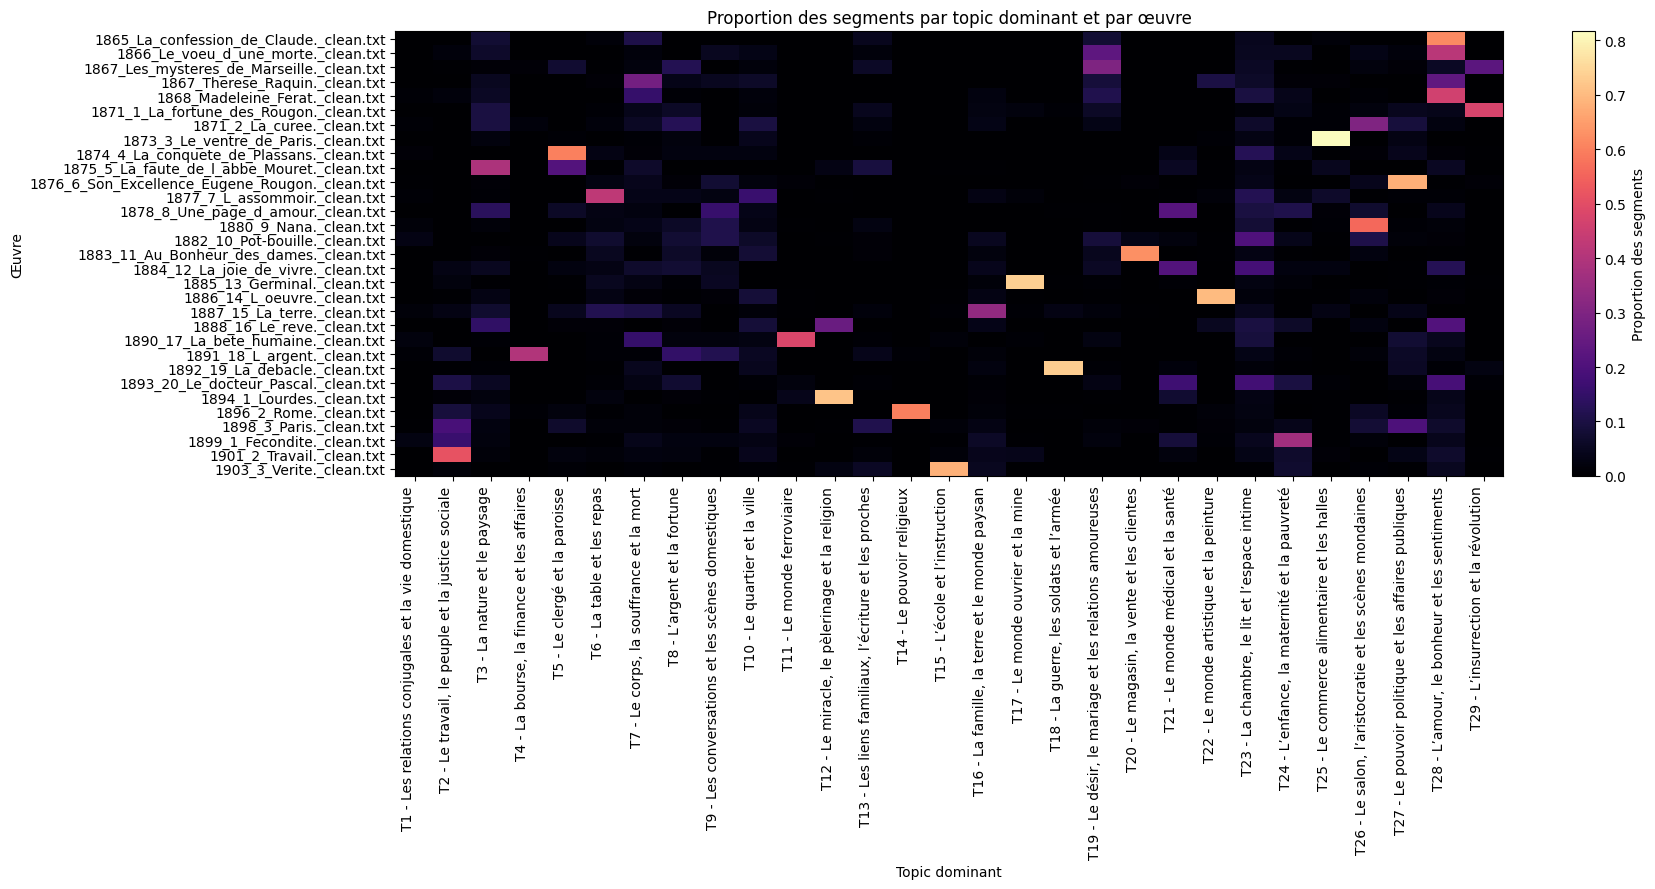
\includegraphics[width=\textwidth]{images/chapitre_1/resultats/proportion_segment_headmap_nmf.png}
    \caption{Heatmap des poids des mots dans les topics NMF}
    \label{fig:heatmap_nmf}
\end{figure}

La heatmap des topics NMF met en évidence une organisation thématique relativement lisible. Certains topics sont associés à des champs lexicaux spécialisés, comme la mine, la finance, la religion, la guerre, le commerce ou le monde ferroviaire. D'autres renvoient à des motifs plus transversaux, comme la famille, l'espace domestique, les sentiments, la maladie ou les relations sociales. Cette visualisation confirme que la NMF produit des regroupements interprétables à partir des poids des mots dans chaque topic.

\begin{figure}[H]
    \centering
    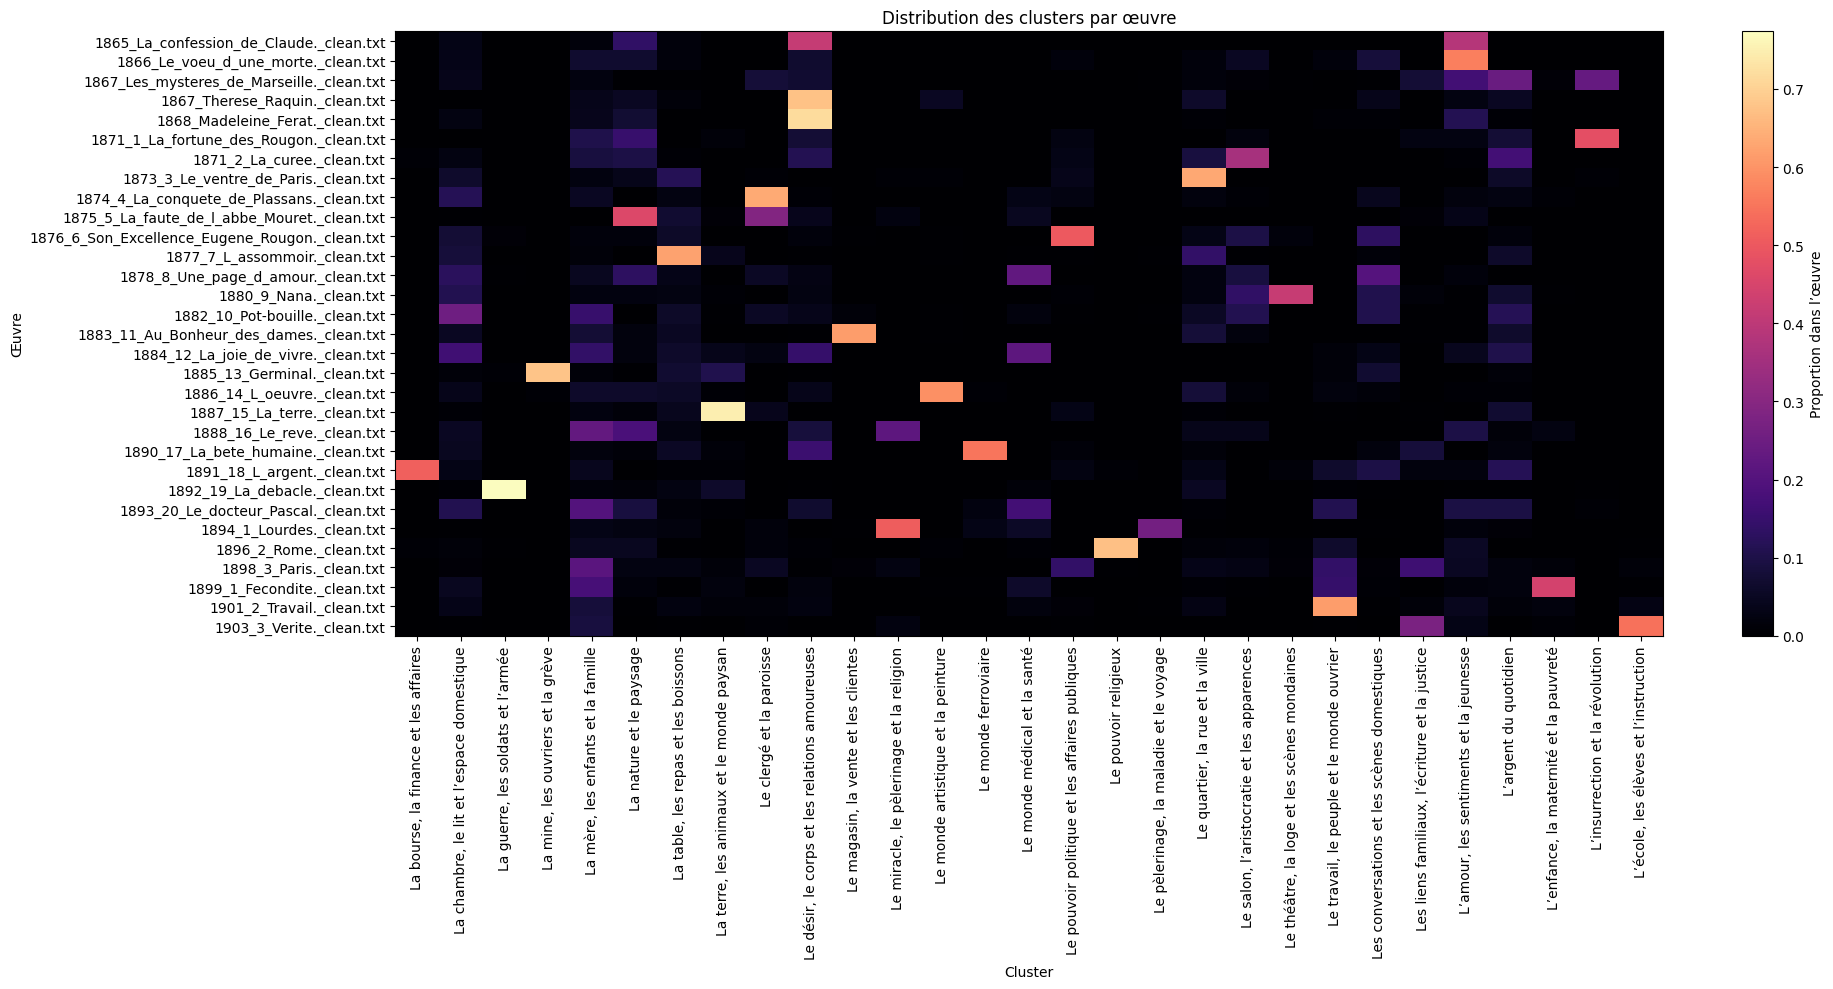
\includegraphics[width=\textwidth]{images/chapitre_1/resultats/headmap_kmeans.png}
    \caption{Heatmap des poids des mots dans les clusters K-means}
    \label{fig:heatmap_kmeans}
\end{figure}

La heatmap des clusters K-means présente une structure comparable, mais avec une logique plus catégorielle. Les mots caractéristiques sont rattachés à des groupes de segments plutôt qu'à des topics latents. On retrouve néanmoins plusieurs ensembles proches de ceux observés avec la NMF : la mine et le monde ouvrier, la bourse et l'argent, le clergé et la religion, la guerre, la ville, le commerce, l'école ou encore l'espace domestique.

La comparaison des deux heatmaps montre donc une convergence partielle entre les méthodes. Certains champs lexicaux apparaissent de manière stable, indépendamment du modèle utilisé. Cette stabilité renforce leur pertinence pour l'analyse du corpus : lorsqu'un même ensemble lexical apparaît à la fois dans les topics NMF et dans les clusters K-means, il devient plus difficile de l'attribuer à un simple effet du modèle. Il s'agit plutôt d'un motif fortement structurant dans le corpus.

Cependant, les deux heatmaps ne doivent pas être interprétées de la même manière. Dans la NMF, les mots caractérisent des topics qui peuvent contribuer simultanément à plusieurs segments. Dans K-means, les mots décrivent le centre lexical de groupes distincts. La NMF donne donc une lecture plus souple des thèmes, tandis que K-means accentue les séparations entre groupes de segments.

\begin{figure}[H]
    \centering
    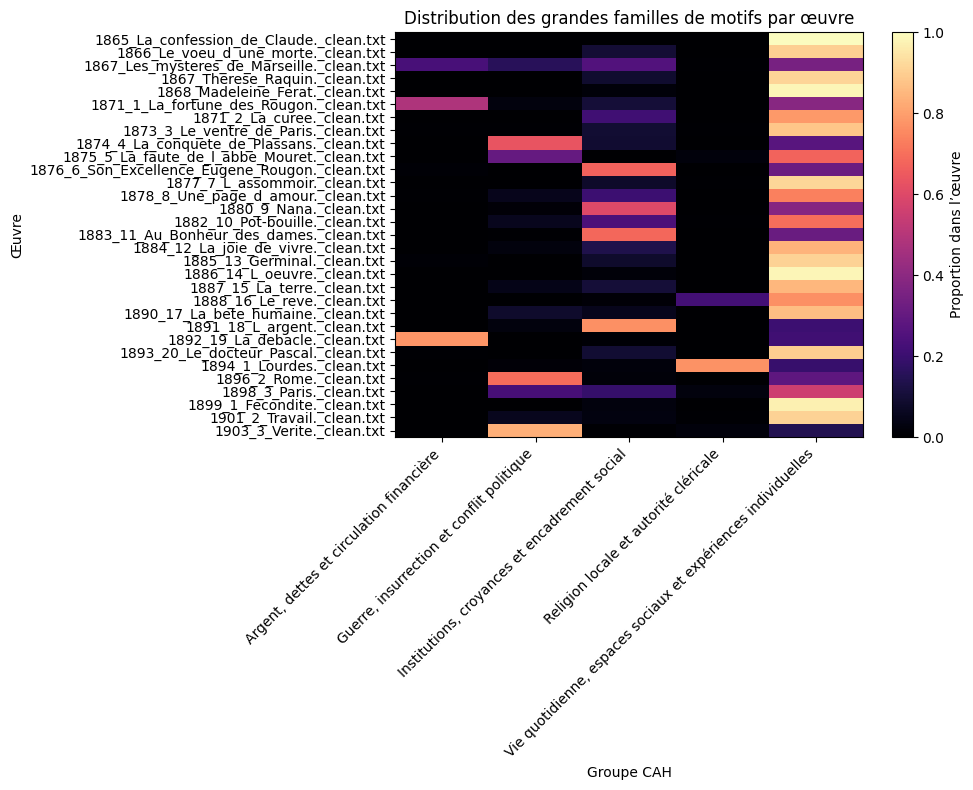
\includegraphics[width=\textwidth]{images/chapitre_1/resultats/grande_famille_kmeans.png}
    \caption{Wordcloud des mots caractéristiques des clusters K-means}
    \label{fig:wordcloud_kmeans}
\end{figure}

Le wordcloud des clusters K-means complète cette lecture en donnant une vue plus synthétique des mots les plus représentatifs des regroupements. Il permet d'observer rapidement les champs lexicaux dominants dans les clusters, mais il reste moins précis que les heatmaps, car il ne montre pas la distribution des mots cluster par cluster. Il doit donc être compris comme une visualisation d'appui, et non comme un outil principal d'interprétation.

\subsection{Convergences thématiques}

Les intitulés attribués aux topics et aux clusters confirment les convergences observées dans les heatmaps. On retrouve, dans les deux méthodes, des ensembles liés au travail, à la mine, à la finance, à la religion, à la famille, au monde domestique, à la guerre, au commerce ou encore aux espaces urbains. Ces convergences indiquent que certains thèmes sont suffisamment présents dans le corpus pour émerger malgré des fonctionnements algorithmiques différents.

Cette convergence n'implique pas que les deux méthodes produisent des résultats identiques. Certains topics NMF peuvent regrouper plusieurs dimensions lexicales que K-means sépare en clusters distincts. Inversement, certains clusters K-means peuvent rassembler des segments proches lexicalement, mais dont l'interprétation thématique reste plus large. La comparaison doit donc porter sur les régularités générales plutôt que sur une correspondance exacte entre chaque topic et chaque cluster.

\subsection{Distribution des thèmes par œuvre}

Afin d'observer la présence des thèmes dans chaque roman, deux visualisations complémentaires ont été produites. La première repose sur les poids moyens normalisés des topics NMF par œuvre. Elle permet d'observer la contribution moyenne de chaque topic dans chaque roman, même lorsque ce topic n'est pas nécessairement dominant dans les segments concernés.

\begin{figure}[H]
    \centering
    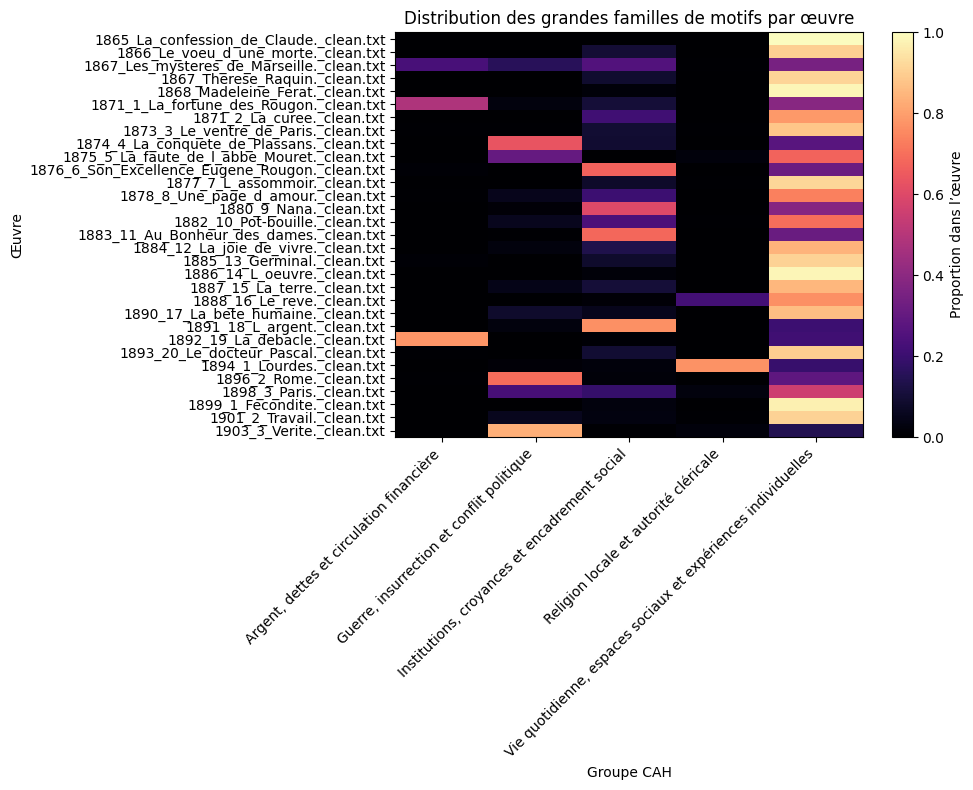
\includegraphics[width=\textwidth]{images/chapitre_1/resultats/grande_famille_kmeans.png}
    \caption{Poids moyen normalisé des topics NMF par œuvre}
    \label{fig:heatmap_poids_topics_nmf_oeuvre}
\end{figure}

Cette première heatmap propose une lecture graduelle de la présence des topics dans les œuvres. Elle permet de repérer les thèmes qui traversent plusieurs romans, mais aussi ceux qui sont plus fortement associés à certaines œuvres. Par exemple, un topic lié à la mine peut être plus visible dans \textit{Germinal}, tandis qu'un topic lié à la finance peut être plus marqué dans \textit{L'Argent}. Cette visualisation est utile parce qu'elle conserve la logique propre à la NMF : un topic peut être présent à des degrés variables dans un même roman.

La seconde visualisation repose sur le topic dominant attribué à chaque segment. Une table croisée a été construite entre les œuvres et les topics dominants, puis normalisée par ligne. Cette normalisation permet d'obtenir, pour chaque roman, la proportion de segments associés à chaque topic dominant. Elle est particulièrement utile pour comparer les œuvres entre elles malgré leurs différences de longueur.

\begin{figure}[H]
    \centering
    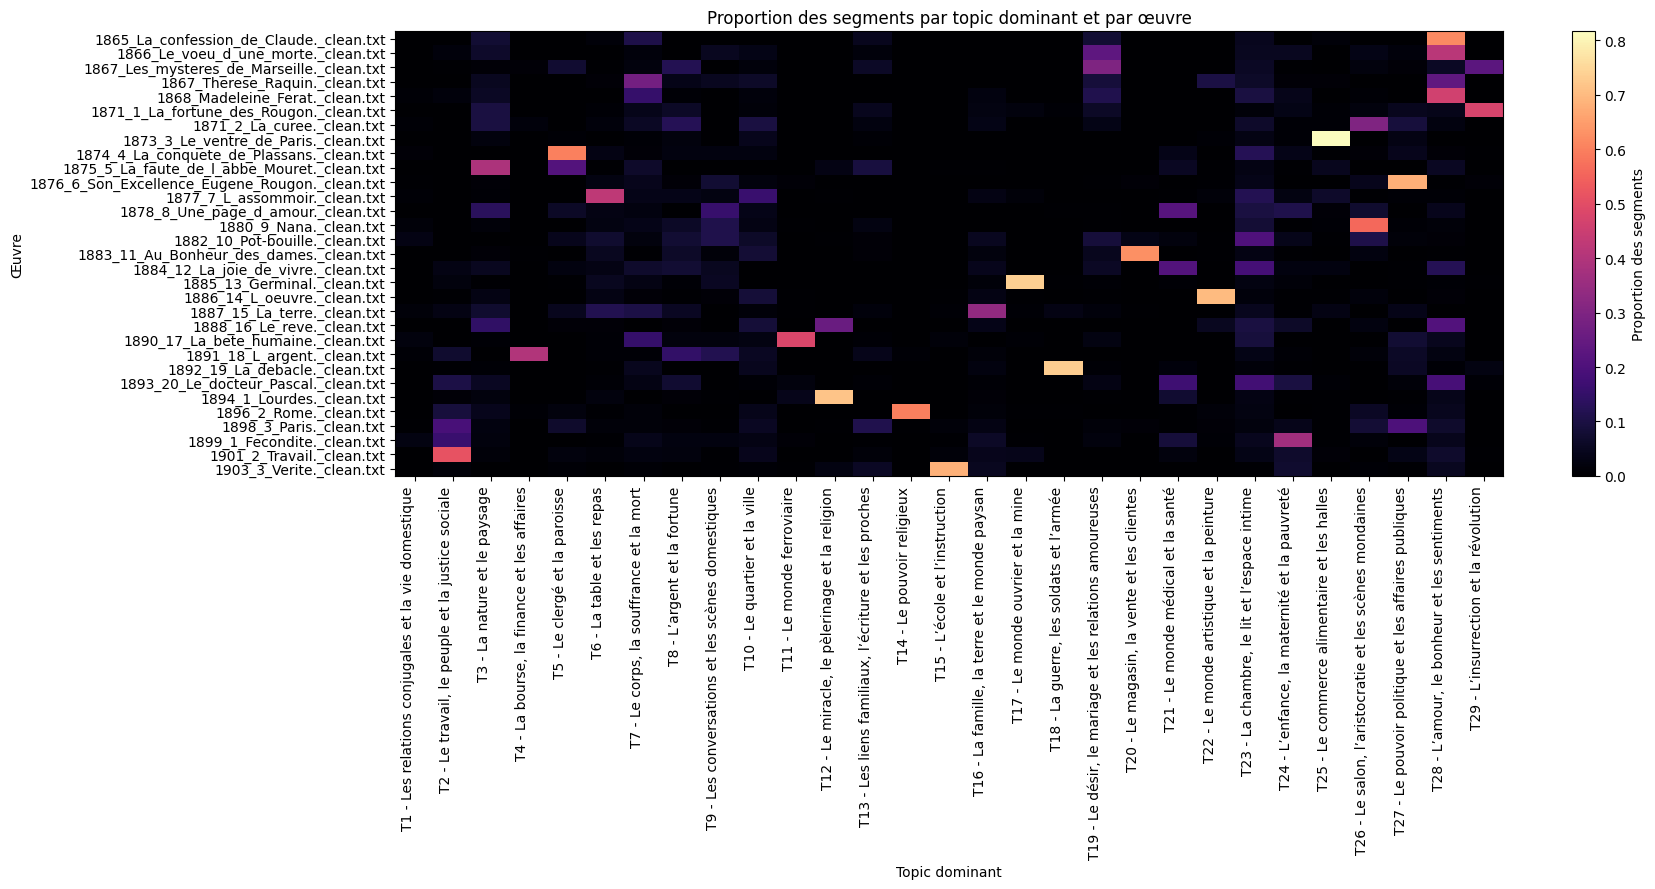
\includegraphics[width=\textwidth]{images/chapitre_1/resultats/proportion_segment_headmap_nmf.png}
    \caption{Proportion des segments par topic dominant et par œuvre}
    \label{fig:heatmap_proportion_topics_oeuvre}
\end{figure}

Cette seconde heatmap donne une lecture plus directement interprétable des thèmes dominants par œuvre. Contrairement à un comptage brut, la normalisation par ligne évite que les romans les plus longs soient mécaniquement surreprésentés. Les zones les plus marquées indiquent les topics qui occupent une place importante dans un roman donné. Cette lecture permet de relier plus facilement certains thèmes à des œuvres précises, comme la mine dans \textit{Germinal}, le commerce dans \textit{Au Bonheur des dames}, la finance dans \textit{L'Argent} ou la guerre dans \textit{La Débâcle}.

Les deux heatmaps ne mesurent donc pas exactement la même chose. La première indique la contribution moyenne des topics dans chaque œuvre, tandis que la seconde montre la proportion de segments pour lesquels un topic est dominant. Leur combinaison permet de distinguer les thèmes diffus, présents à faible intensité dans de nombreux segments, des thèmes plus structurants, qui dominent nettement certains passages ou certaines œuvres.

\subsection{Apport de la double approche}

La comparaison entre NMF et K-means montre l'intérêt d'une double approche. La NMF offre une lecture souple et graduelle des thèmes, tandis que K-means propose une classification plus nette des segments. Le croisement des deux méthodes permet donc de mieux distinguer les thèmes stables de ceux qui dépendent davantage du modèle utilisé.

Ainsi, K-means ne remplace pas la NMF, mais il constitue un complément méthodologique utile. Lorsque les deux méthodes font apparaître des champs lexicaux proches, l'interprétation gagne en solidité. Lorsqu'elles divergent, ces écarts invitent au contraire à examiner plus précisément les segments concernés et à nuancer l'interprétation. Cette double lecture permet donc de renforcer l'analyse tout en conservant une part d'interprétation qualitative indispensable dans l'étude d'un corpus littéraire.